\documentclass[a4paper]{article}
\usepackage[french]{babel}
\usepackage[utf8]{inputenc}
\usepackage[T1]{fontenc}
\usepackage{hyperref}
\usepackage{graphicx}
\usepackage{appendix}
\usepackage{caption}
\usepackage{pdfpages}
\usepackage{mathtools}
\usepackage{cite}
\usepackage{array}
\usepackage{multirow}
\usepackage{listings}
\lstset{language=Python}
\begin{document}

\begin{titlepage}
\newcommand{\HRule}{\rule{\linewidth}{0.5mm}} 
\center 
 
%----------------------------------------------------------------------------------------
%	HEADING SECTIONS
%----------------------------------------------------------------------------------------

\textsc{\LARGE Université de Bordeaux}\\[1.5cm] 
\textsc{\Large Projet Métaheuristique}\\[0.5cm] 
\textsc{\large M1 Informatique}\\[0.5cm] 

%----------------------------------------------------------------------------------------
%	TITLE SECTION
%----------------------------------------------------------------------------------------

\HRule \\[0.4cm]
{ \huge \bfseries Partitionnement de graphe en K classes}\\[0.4cm] % Title of your document
\HRule \\[1.5cm]
 
%----------------------------------------------------------------------------------------
%	AUTHOR SECTION
%----------------------------------------------------------------------------------------

\begin{minipage}{0.4\textwidth}
\begin{flushleft} \large
\emph{Auteurs : }\\
Norbert \textsc{Feron},\\
Baptiste \textsc{Masset}
\end{flushleft}
\end{minipage}
~
\begin{minipage}{0.4\textwidth}
\begin{flushright} \large
\emph{Encadrant : } \\
Marc Michel \textsc{Corsini} 
\end{flushright}
\end{minipage}\\[2cm]

%----------------------------------------------------------------------------------------
%	DATE SECTION
%----------------------------------------------------------------------------------------

{\large \today}\\[2cm]

%----------------------------------------------------------------------------------------
%	LOGO SECTION
%----------------------------------------------------------------------------------------


\includegraphics{img/logo.png}\\[1cm]
 
%----------------------------------------------------------------------------------------

\vfill
\end{titlepage}
%----------------------------------------------------------------------------------------

\tableofcontents

\newpage

\section{Introduction}
Dans le cadre de l'UE Graphes et Recherche Opérationnel du Master 1 Informatique de l'Université de Bordeaux, nous avons mis en œuvre ce projet qui a pour but de mettre en pratique des heuristiques et méta-heuristiques, tels que la descente de gradient, le recuit simulé ou encore la méthode tabou, sur un problème de partitionnement de graphe. Pour cela nous disposons de graphes pondérés, de différentes tailles (de cinq sommets à plus de milles), sur lesquelles nous allons tester et comparer les résultats de nos différents algorithmes appliqués au problème de partitionnement de graphe en K classes ``à peu près équitables''.

	\subsection{Définition d'une méta-heuristique}
	\begin{textit}
	Une méta-heuristique est un algorithme d’optimisation visant à résoudre des problèmes d’optimisation difficile (souvent issus des domaines de la recherche opérationnelle, de l'ingénierie ou de l'intelligence artificielle) pour lesquels on ne connaît pas de méthode classique plus efficace.
	\end{textit}

	Les méta-heuristiques sont généralement des algorithmes stochastiques itératifs, qui progressent vers un optimum global, c'est-à-dire l'extremum global d'une fonction, par échantillonnage d’une fonction objectif. Elles se comportent comme des algorithmes de recherche, tentant d’apprendre les caractéristiques d’un problème afin d’en trouver une approximation de la meilleure solution.

	\subsection{Problématique}
	Notre problème est le suivant : partitionner un graphe en K classes ``à peu près équitable'' tout en minimisant le poids des arêtes interclasses. En d'autres termes, cela consiste à placer chaque sommet du graphe dans une des classe de manières à minimiser la somme des poids des arrêtes n'appartenant pas à la même classe.
	\begin{center}
	min($\sum\limits_{i} \sum\limits_{j}  \omega (i,j)$)
	\end{center}
	avec $i \in K1, j \in K2, i \ne j$ et $\omega (i,j)$ le poids entre $i$ et $j$.

	\subsection{Nombre de classes}
	En ce qui concerne le nombre de classes en lequel vont être partitionnés nos graphes, nous avons choisi de laisser ce paramètre externe au problème. Autrement dit, c'est à l'utilisateur de définir ce paramètre à l’exécution suivant le nombre de sommets du graphe et ses attentes.
	Aussi le nombre de solutions potentielles vaut $k^n$ avec $k$ le nombre de classes et $n$ le nombre de sommets du graphe. 

	Attention donc à ne pas choisir un $k$ trop grand pour un graphe comportant beaucoup de sommets au risque de ne pas avoir de retour du programme en un temps raisonnable. 

	\subsection{Définition de l'équité}

	Pour ce qui est de la notion d' ``à peu près équitables'' entre les classes, nous avons choisi de laisser ce paramètre à l'appréciation de l'utilisateur par soucis de généricité. Celui-ci dispose d'une variable supplémentaire appelée ``delta\_max''. Cette variable correspond à l'écart maximum d'éléments autorisé entre les classes pour qu'une solution soit considérée comme acceptable et puisse être retournée en sortie des différents algorithmes utilisés dans ce projet.

	De plus, le score des solutions est pénalisé par la différence du nombre de sommets dans les classes par une constante appelé $\mu$ ``mu'' $\in [0,1]$. Ainsi, plus la disparité entre les classes sera grande plus la pénalité sera élevée.

	\subsection{Fonction objectif}
	Cette fonction permet de décrire la qualité d'une solution.


	L'objectif du projet est de minimiser la somme du poids des arrêtes interclasses, nous retenons donc les solutions dont le score est le plus faible. Le calcul du score est : 
	\begin{center}
	$\sum\limits_{i} \sum\limits_{j}  \omega (i,j)) + \mu * c(\delta)$
	\end{center}
	avec $i \in K1, j \in K2, i \ne j$, $\omega (i,j)$ le poids entre $i$ et $j$, $\mu$ une constante $\in [0,1]$, $\delta$ l'écart en terme d'éléments entre K1 et K2 et $c(\delta)$ le rapport entre $\delta$ et le nombre total de sommets.

\section{Méthode d’énumération}
La solution la plus simple consiste à énumérer toutes les solutions valides et de calculer la somme du poids des arrêtes interclasses, les solutions avec le meilleur score sont retournées en résultats de l'algorithme d'énumération. Les solutions retournées sont donc toujours les solutions optimales, cependant la puissance de nos calculateurs fait défaut et en dépassant un certain nombre de sommets, nos ordinateurs ne disposent pas d'un puissance de calcul suffisante et l'énumération des solutions devient impossible à effectuer en un temps raisonnable.

\section{L'espace de recherche}
Lors de l'utilisation des méta-heuristiques, l'ensemble des solutions possibles forment un espace de recherche borné. Le but de nos méta-algorithmes est donc de trouver l'optimum global, c'est à dire la meilleure solution au problème.
	\subsection{Notion de voisinage}
	Le voisinage d'une solution est l’ensemble des solutions voisines, c’est à dire l’ensemble des solutions accessibles par un mouvement et un seul. Afin de trouver la solution optimale nous allons donc répéter l'évaluation du voisinage d'une solution.
	\subsection{Mouvement élémentaire}
	Un mouvement est une opération élémentaire permettant de passer d’une solution à une
solution voisine. Ce mouvement nous permet donc de créer le voisinage d'une solution. Trois mouvement différents ont été utilisés dans ce projet, à savoir :
\begin{enumerate}
\item{Pick'n'Drop : prend un élément d'une classe et le dépose dans une autre}
\item{Swap : échange deux éléments}
\item{Sweep : permutation circulaire des éléments}
\end{enumerate}

\section{Descente de Gradient (glouton)}
	\subsection{Algorithme glouton}
	Un algorithme glouton est un algorithme qui construit sa solution pas à pas, sans revenir sur ses décisions et en effectuant à chaque étape le choix qui semble le meilleur.

	L'hypothèse pour ce type d'algorithme est que des choix locaux optimaux successifs produisent un résultat global optimal. Il a pour avantage d'avoir une faible complexité et d'être rapide.

	\subsection{Fonctionnement}
	La descente de gradient (ou hillclimbing) est la méthode d'optimisation stochastique la plus simple et fonctionne de cette manière :
	\begin{enumerate}
		\item{Choisir un point de départ (aléatoirement ou non)}
		\item{À chaque étape, prendre la première solution voisine améliorante}
		\item{S'il n'y a plus de solution améliorante; stop; sinon revenir à l'étape 2}
	\end{enumerate}

	On peut assimiler cette algorithme à un alpiniste cherchant à grimper (ou descendre) une montagne une étape après l'autre. C'est un algorithme glouton car il ne prend que des solutions améliorante, qui font monter (ou descendre) notre alpiniste. Nous arrivons donc rapidement en haut (ou en bas) de la colline, cependant rien ne nous assure que cette colline soit la plus haute (ou la plus basse).


	\noindent%
	\begin{minipage}{\linewidth}% to keep image and caption on one page
	\makebox[\linewidth]{%        to center the image
	  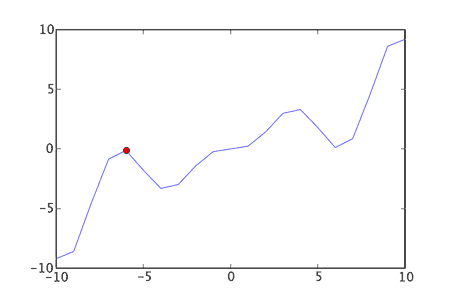
\includegraphics[keepaspectratio=true,scale=0.7]{img/hc.png}}
	\captionof{figure}{Représentation d'un espace de recherche}\label{hc}%      only if needed  
	\end{minipage}\\

	Comme vous pouvez le voir sur cette figure, notre solution courante (le point rouge) ne peux plus qu'aller en descendant, pourtant ce n'est pas le plus au point du paysage.

	Le plus haut point correspond à l'optimum global et le point rouge correspond à l'optimum local.

	C'est donc la limite, cette algorithme tend à rester coincé dans son optimum local. Une variante de cette algorithme consiste à le faire redémarrer tant que le nombre d'évaluation maximum définit par l'utilisateur n'est pas atteint en choisissant un nouveau point de départ.\\\\

	Dans la suite nous verrons des méta-algorithme qui eux ont la particularité de ne pas rester coincés dans un optimum local, et donc trouvent toujours l'optimum global, ou du moins s'en approche.
\section{Recuit Simulé}
Tout droit sortie de la thermodynamique et plus précisément d'un phénomène en métallurgie, le recuit simulé ressemble à une descente de gradient mais avec la capacité de sortir des optimum locaux.

Cette capacité est due à l'introduction de deux nouvelles variable, un température et un coefficient de refroidissement.

	\subsection{Fonctionnement}
	\begin{enumerate}
		\item{Choisir un point de départ (aléatoirement ou non)}
		\item{Définir une température initiale et un coefficient de refroidissement}
		\item{Choisir le premier voisin de la solution courante}
		\begin{itemize}
			\item{Si ce voisin est améliorant, on le choisit comme solution courante}
			\item{Si ce voisin est moins bon, choisir de manière probabiliste d'en faire la solution courante en se basant sur la température courante et son niveau de ``moins bon''}
		\end{itemize}
		\item{Baisser la température}
		\item{Revenir à l'étape 3}
	\end{enumerate}

En baissant doucement la température, nous avons moins de chance de choisir une solution non améliorante au cours du temps. Quand la température est vraiment basse, on revient à la descente de gradient.
Le choix probabiliste de prendre une solution ou non se fait grâce à l’algorithme de Métropolis.

L'inconvénient de cette algorithme réside dans le choix des paramètre de température et de refroidissement, souvent définie de manière empirique. 


\section{Recherche Tabou}
La recherche tabou est une amélioration de la descente de gradient. En effet, le fonctionnement est le même en tout point à l'exception près de l'introduction d'une file de taille définie, nous permettant de stocker la solution précédente à la solution courante. Ainsi nous évitons de repasser par un voisin déjà visité. Ce mécanisme permet donc à la descente de gradient de sortir d'un optimum local.

	\subsection{Fonctionnement}
	\begin{enumerate}
		\item{Choisir un point de départ (aléatoirement ou non)}
		\item{À chaque étape, prendre la première solution voisine améliorante}
		\item{Si elle n'est pas dans la pile; en faire la solution courante et stocker son prédécesseur dans la pile; sinon choisir une autre solution voisine améliorante}
		\item{S'il n'y a plus de solution améliorante; stop; sinon revenir à l'étape 2}
	\end{enumerate}

Plusieurs stratégies sont possibles, stocker son prédécesseur, stocker le mouvement nous ayant permis d'arriver à la solution...
Ici la pile est une mémoire à court terme (ne pas excéder une taille de 15), mais nous pourrions mettre en place différent type de mémoire. \\

Aussi le critère d'arrêt, comme pour les méta-algorithmes précédents, peuvent différer. Soit on s'arrête lorsque le nombre maximum d'itération est atteint, lorsque aucune solution améliorante n'a été trouvée depuis un certain temps, lorsque la variation des solutions est trop faible, lorsque la température dans le cas du recuit simulé est trop basse...

\section{Comparaison des trois mouvements élémentaires}
Nous allons maintenant comparer les trois mouvements élémentaires nous permettant de construire le voisinage : Pick'n'Drop, Swap, Sweep.
Les tests ont été effectués sur un graphe à 30 sommets en 2 classes avec un maximum de 3 éléments d'écart entre les classes.
	\subsection{Descente de Gradient}
		\begin{verbatim}
INFO:multi_proc.mproc_hillclimb:-------MULTI_PROC HILLCLIMB-------
INFO:multi_proc.mproc_hillclimb:Running on 8 proc
INFO:multi_proc.mproc_hillclimb:nbS = 30; nbK = 2; delta_max = 3; mu = 1.0;
move_operator=pick_gen
INFO:multi_proc.mproc_hillclimb:for 100 iteration with 100 max_evaluations each, 
 total time in sec : 5.6474458440206945
 best score found is 188,
 mean time in sec : 0.41084918993961766,
 mean best_score : 193.66666666666669, EcT : 2.9370499870214375
 mean num_eval : 51.84

 INFO:multi_proc.mproc_hillclimb:-------MULTI_PROC HILLCLIMB-------
INFO:multi_proc.mproc_hillclimb:Running on 8 proc
INFO:multi_proc.mproc_hillclimb:nbS = 30; nbK = 2; delta_max = 3; mu = 1.0;
move_operator=swap_gen
INFO:multi_proc.mproc_hillclimb:for 100 iteration with 100 max_evaluations each, 
 total time in sec : 13.165540570014855
 best score found is 190,
 mean time in sec : 0.9277846304691048,
 mean best_score : 194.82533333333333, EcT : 2.039140682990769
 mean num_eval : 100.0

 INFO:multi_proc.mproc_hillclimb:-------MULTI_PROC HILLCLIMB-------
INFO:multi_proc.mproc_hillclimb:Running on 8 proc
INFO:multi_proc.mproc_hillclimb:nbS = 30; nbK = 2; delta_max = 3; mu = 1.0;
move_operator=sweep_gen
INFO:multi_proc.mproc_hillclimb:for 100 iteration with 100 max_evaluations each, 
 total time in sec : 13.09051345998887
 best score found is 189,
 mean time in sec : 0.9137671065484756,
 mean best_score : 194.7413333333333, EcT : 2.4469827042007655
 mean num_eval : 100.0
		\end{verbatim}
	\subsection{Recuit Simulé}
		\begin{verbatim}
INFO:multi_proc.mproc_anneal:-------MULTI_PROC SIMULATED ANNEALING-------
INFO:multi_proc.mproc_anneal:Running on 8 proc
INFO:multi_proc.mproc_anneal:nbS = 30; nbK = 2; delta_max = 3; mu = 1.0; 
final_temp = 1.4159869113351014; alpha = 0.95; move_operator= pick_gen
INFO:multi_proc.mproc_anneal:for 100 iteration with 100 max_evaluations each, 
 best score found is 193,
 total time in sec : 14.668629520980176
 mean time in sec : 1.023166321387398,
 mean best_score : 197.67666666666668, EcT : 2.0977541301526235
 mean num_eval : 100.0,
 mean end temperature : 1.2664165177126414

 INFO:multi_proc.mproc_anneal:-------MULTI_PROC SIMULATED ANNEALING-------
INFO:multi_proc.mproc_anneal:Running on 8 proc
INFO:multi_proc.mproc_anneal:nbS = 30; nbK = 2; delta_max = 3; mu = 1.0; 
final_temp = 1.4159869113351014; alpha = 0.95; move_operator= swap_gen
INFO:multi_proc.mproc_anneal:for 100 iteration with 100 max_evaluations each, 
 best score found is 193,
 total time in sec : 37.858596491016215
 mean time in sec : 2.5797699854095115,
 mean best_score : 198.18266666666668, EcT : 2.5924282391387767
 mean num_eval : 100.0,
 mean end temperature : 1.4003589296125034

 INFO:multi_proc.mproc_anneal:-------MULTI_PROC SIMULATED ANNEALING-------
 INFO:multi_proc.mproc_anneal:Running on 8 proc
INFO:multi_proc.mproc_anneal:nbS = 30; nbK = 2; delta_max = 3; mu = 1.0; 
final_temp = 1.2779281874799289; alpha = 0.95; move_operator= sweep_gen
INFO:multi_proc.mproc_anneal:for 100 iteration with 100 max_evaluations each, 
 best score found is 194,
 total time in sec : 39.423500056989724
 mean time in sec : 2.7440948232493247,
 mean best_score : 198.33, EcT : 2.223784804161333
 mean num_eval : 100.0,
 mean end temperature : 1.3372233881087228
		\end{verbatim}
	\subsection{Recherche Tabou}
		\begin{verbatim}
INFO:multi_proc.mproc_tabu:-------MULTI_PROC TABUSEARCH-------
INFO:multi_proc.mproc_tabu:Running on 8 proc
INFO:multi_proc.mproc_tabu:nbS = 30; nbK = 2; delta_max = 3; mu = 1.0;
move_operator=pick_gen; tabu_maxsize = 15
INFO:multi_proc.mproc_tabu:for 100 iteration with 100 max_evaluations each, 
 total time in sec : 5.805855156009784
 best score found is 189,
 mean time in sec : 0.42773062509309967,
 mean best_score : 193.40666666666667, EcT : 2.6216657516036084
 mean num_eval : 9.96

 INFO:multi_proc.mproc_tabu:-------MULTI_PROC TABUSEARCH-------
INFO:multi_proc.mproc_tabu:Running on 8 proc
INFO:multi_proc.mproc_tabu:nbS = 30; nbK = 2; delta_max = 3; mu = 1.0;
move_operator=swap_gen; tabu_maxsize = 15
INFO:multi_proc.mproc_tabu:for 100 iteration with 100 max_evaluations each, 
 total time in sec : 68.0415397619945
 best score found is 188,
 mean time in sec : 4.820201046710135,
 mean best_score : 190.21466666666666, EcT : 1.4176245127886513
 mean num_eval : 9.93

 INFO:multi_proc.mproc_tabu:-------MULTI_PROC TABUSEARCH-------
INFO:multi_proc.mproc_tabu:Running on 8 proc
INFO:multi_proc.mproc_tabu:nbS = 30; nbK = 2; delta_max = 3; mu = 1.0;
move_operator=sweep_gen; tabu_maxsize = 15
INFO:multi_proc.mproc_tabu:for 100 iteration with 100 max_evaluations each, 
 total time in sec : 61.12722033701721
 best score found is 188,
 mean time in sec : 4.582537554161681,
 mean best_score : 190.05533333333332, EcT : 1.4300621979519719
 mean num_eval : 9.66
		\end{verbatim}
\\

En ne faisant varier que le type de mouvement élémentaire, on remarque que la différence la plus notable est le temps. En effet, on remarque que quelque soit la méta-heuristique utilisée, le mouvement Pick'n'Drop est nettement plus efficace. 

De 5 secondes à 60 secondes dans le cas de la recherche tabou.
\section{Test \& Résultats}
Nous avons testé nos algorithmes sur des graphes allant de 4 sommets à 100 sommets, les méta-algorithmes de descente de gradient, recuit simulé et recherche tabou sont lancés de manière indépendante et en parallèle sur le nombre de cœurs disponible sur la machine. Après un nombre d'itérations (fixé à 100 pour nos tests), on calcul les statistiques associées à chaque algorithme.

L'énumération ne nécessite pas d'itérations car elle fournie toujours les mêmes résultats, à savoir la ou les meilleurs solutions.

Voici nos résultats:

\subsection{Algorithme d'énumération}
\subsubsection{4 Sommets en 2 classes, mu = [1; 0.5; 0]}
\begin{verbatim}
-------ENUMERATE-------
nbS = 4; nbK = 2; delta_max = 3; mu = 1.0
best score is : 1,
 total time : 0.00038140779361128807
-------ENUMERATE-------
nbS = 4; nbK = 2; delta_max = 3; mu = 0.5
best score is : 1,
 total time : 0.00037381192669272423
-------ENUMERATE-------
nbS = 4; nbK = 2; delta_max = 3; mu = 0.0
best score is : 1,
 total time : 0.0003458610735833645
\end{verbatim}
\subsubsection{5 Sommets en 2 classes, mu = [1; 0.5; 0]}
\begin{verbatim}
-------ENUMERATE-------
nbS = 5; nbK = 2; delta_max = 3; mu = 1.0
best score is : 3,
 total time : 0.0008135139942169189
-------ENUMERATE-------
nbS = 5; nbK = 2; delta_max = 3; mu = 0.5
best score is : 3,
 total time : 0.0008682990446686745
-------ENUMERATE-------
nbS = 5; nbK = 2; delta_max = 3; mu = 0.0
best score is : 3,
 total time : 0.0007814168930053711
\end{verbatim}
\subsubsection{20 Sommets en 2 classes, mu = [1; 0.5; 0]}
\begin{verbatim}
-------ENUMERATE-------
nbS = 20; nbK = 2; delta_max = 3; mu = 1.0
best score is : 39,
 total time : 163.1898413640447
-------ENUMERATE-------
nbS = 20; nbK = 2; delta_max = 3; mu = 0.5
best score is : 39,
 total time : 160.39260955667123
-------ENUMERATE-------
nbS = 20; nbK = 2; delta_max = 3; mu = 0.0
best score is : 39,
 total time : 164.47484961291775
\end{verbatim}

\subsection{Descente de Gradient}
\subsubsection{5 Sommets en 2 classes, mu = [1; 0.5; 0]}
\begin{verbatim}
-------MULTI_PROC HILLCLIMB-------
Running on 16 proc
nbS = 5; nbK = 2; delta_max = 3; mu = 1.0; move_operator= pick_gen
for 100 iteration with 100 max_evaluations each, 
 total time in sec : 0.10310757299885154
 best score found is 3,
 mean time in sec : 0.001071562976576388,
 mean best_score : 3.63, EcT : 0.1714466079977652
 mean num_eval : 7.07
-------MULTI_PROC HILLCLIMB-------
Running on 16 proc
nbS = 5; nbK = 2; delta_max = 3; mu = 0.5; move_operator= pick_gen
for 100 iteration with 100 max_evaluations each, 
 total time in sec : 0.10206909896805882
 best score found is 3,
 mean time in sec : 0.0012981305923312903,
 mean best_score : 3.36, EcT : 0.23868325657594203
 mean num_eval : 6.82
-------MULTI_PROC HILLCLIMB-------
Running on 16 proc
nbS = 5; nbK = 2; delta_max = 3; mu = 0.0; move_operator= pick_gen
for 100 iteration with 100 max_evaluations each, 
 total time in sec : 0.10367809794843197
 best score found is 3,
 mean time in sec : 0.0010838805558159947,
 mean best_score : 3.05, EcT : 0.2190429135575903
 mean num_eval : 6.94
\end{verbatim}
\subsubsection{15 Sommets en 3 classes, mu = [1; 0.5; 0]}
\begin{verbatim}
-------MULTI_PROC HILLCLIMB-------
Running on 16 proc
nbS = 15; nbK = 3; delta_max = 3; mu = 1.0; move_operator= pick_gen
for 100 iteration with 100 max_evaluations each, 
 total time in sec : 0.2024659407325089
 best score found is 58,
 mean time in sec : 0.023689089985564352,
 mean best_score : 61.010000000000005, EcT : 1.1520293907586374
 mean num_eval : 21.36
-------MULTI_PROC HILLCLIMB-------
Running on 16 proc
nbS = 15; nbK = 3; delta_max = 3; mu = 0.5; move_operator= pick_gen
for 100 iteration with 100 max_evaluations each, 
 total time in sec : 0.20349178183823824
 best score found is 58,
 mean time in sec : 0.024920869143679737,
 mean best_score : 61.01, EcT : 1.2956414892580694
 mean num_eval : 21.34
-------MULTI_PROC HILLCLIMB-------
Running on 16 proc
nbS = 15; nbK = 3; delta_max = 3; mu = 0.0; move_operator= pick_gen
for 100 iteration with 100 max_evaluations each, 
 total time in sec : 0.2024315781891346
 best score found is 59,
 mean time in sec : 0.020131065961904823,
 mean best_score : 61.58, EcT : 1.464599093626138
 mean num_eval : 18.2
\end{verbatim}
\subsubsection{20 Sommets en 3 classes, mu = [1; 0.5; 0]}
\begin{verbatim}
-------MULTI_PROC HILLCLIMB-------
Running on 16 proc
nbS = 20; nbK = 3; delta_max = 3; mu = 1.0; move_operator= pick_gen
for 100 iteration with 100 max_evaluations each, 
 total time in sec : 0.9040888692252338
 best score found is 53,
 mean time in sec : 0.11574626796413214,
 mean best_score : 56.768, EcT : 1.9256052439572229
 mean num_eval : 90.18
-------MULTI_PROC HILLCLIMB-------
Running on 16 proc
nbS = 20; nbK = 3; delta_max = 3; mu = 0.5; move_operator= pick_gen
for 100 iteration with 100 max_evaluations each, 
 total time in sec : 0.8043653820641339
 best score found is 53,
 mean time in sec : 0.11241874734871089,
 mean best_score : 56.617000000000004, EcT : 1.7737026842515662
 mean num_eval : 90.2
-------MULTI_PROC HILLCLIMB-------
Running on 16 proc
nbS = 20; nbK = 3; delta_max = 3; mu = 0.0; move_operator= pick_gen
for 100 iteration with 100 max_evaluations each, 
 total time in sec : 0.8047608300112188
 best score found is 53,
 mean time in sec : 0.09706705980934202,
 mean best_score : 57.68, EcT : 2.3989896863370452
 mean num_eval : 80.08
\end{verbatim}
\subsubsection{50 Sommets en 3 classes, mu = [1; 0.5; 0]}
\begin{verbatim}
-------MULTI_PROC HILLCLIMB-------
Running on 16 proc
nbS = 50; nbK = 3; delta_max = 3; mu = 1.0; move_operator= pick_gen
for 100 iteration with 100 max_evaluations each, 
 total time in sec : 14.029909709934145
 best score found is 288,
 mean time in sec : 2.0499937719944863,
 mean best_score : 310.6014, EcT : 7.05828047563479
 mean num_eval : 100
-------MULTI_PROC HILLCLIMB-------
Running on 16 proc
nbS = 50; nbK = 3; delta_max = 3; mu = 0.5; move_operator= pick_gen
for 100 iteration with 100 max_evaluations each, 
 total time in sec : 14.246775717940181
 best score found is 292,
 mean time in sec : 2.059209058196284,
 mean best_score : 312.4839, EcT : 6.499423112706218
 mean num_eval : 100
-------MULTI_PROC HILLCLIMB-------
Running on 16 proc
nbS = 50; nbK = 3; delta_max = 3; mu = 0.0; move_operator= pick_gen
for 100 iteration with 100 max_evaluations each, 
 total time in sec : 13.881034784018993
 best score found is 294,
 mean time in sec : 2.0022386860102417,
 mean best_score : 310.4, EcT : 6.935489175322106
 mean num_eval : 100
\end{verbatim}
\subsubsection{100 Sommets en 4 classes, mu = [1; 0.5; 0]}
\begin{verbatim}
-------MULTI_PROC HILLCLIMB-------
Running on 16 proc
nbS = 100; nbK = 4; delta_max = 3; mu = 1.0; move_operator= pick_gen
for 100 iteration with 100 max_evaluations each, 
 total time in sec : 275.9682481228374
 best score found is 1430,
 mean time in sec : 40.02110815170687,
 mean best_score : 1476.0958, EcT : 14.049210494371259
 mean num_eval : 100
-------MULTI_PROC HILLCLIMB-------
Running on 16 proc
nbS = 100; nbK = 4; delta_max = 3; mu = 0.5; move_operator= pick_gen
for 100 iteration with 100 max_evaluations each, 
 total time in sec : 278.2741830400191
 best score found is 1451,
 mean time in sec : 40.016724326196126,
 mean best_score : 1475.13245, EcT : 12.389276001686275
 mean num_eval : 100
-------MULTI_PROC HILLCLIMB-------
Running on 16 proc
nbS = 100; nbK = 4; delta_max = 3; mu = 0.0; move_operator= pick_gen
for 100 iteration with 100 max_evaluations each, 
 total time in sec : 274.8639584830962
 best score found is 1444,
 mean time in sec : 39.720520393801856,
 mean best_score : 1472.87, EcT : 13.68967390835778
 mean num_eval : 100
\end{verbatim}

\subsection{Recuit Simulé}
\subsubsection{5 Sommets en 2 classes, mu = [1; 0.5; 0]}
\begin{verbatim}
-------MULTI_PROC SIMULATED ANNEALING-------
Running on 16 proc
nbS = 5; nbK = 2; delta_max = 3; mu = 1.0;
; start_temp = 100; final_temp = 0.89242491504672; alpha = 0.95; move_operator= pick_gen
for 100 iteration with 100 max_evaluations each, 
 best score found is 3,
 total time in sec : 0.15890276758000255
 mean time in sec : 0.019896002300083638,
 mean best_score : 3.6, EcT : 0.0
 mean num_eval : 100,
 mean end temperature : 1.0925721940968705
-------MULTI_PROC SIMULATED ANNEALING-------
Running on 16 proc
nbS = 5; nbK = 2; delta_max = 3; mu = 0.5;
; start_temp = 100; final_temp = 1.2779281874799289; alpha = 0.95; move_operator= pick_gen
for 100 iteration with 100 max_evaluations each, 
 best score found is 3,
 total time in sec : 0.14763296116143465
 mean time in sec : 0.019895954332314433,
 mean best_score : 3.3, EcT : 0.0
 mean num_eval : 100,
 mean end temperature : 1.1712864838845436
-------MULTI_PROC SIMULATED ANNEALING-------
Running on 16 proc
nbS = 5; nbK = 2; delta_max = 3; mu = 0.0;
; start_temp = 100; final_temp = 1.3451875657683463; alpha = 0.95; move_operator= pick_gen
for 100 iteration with 100 max_evaluations each, 
 best score found is 3,
 total time in sec : 0.135501594748348
 mean time in sec : 0.018298799749463798,
 mean best_score : 3.0, EcT : 0.0
 mean num_eval : 100,
 mean end temperature : 1.2735855241323177
\end{verbatim}
\subsubsection{15 Sommets en 3 classes, mu = [1; 0.5; 0]}
\begin{verbatim}
-------MULTI_PROC SIMULATED ANNEALING-------
Running on 16 proc
nbS = 15; nbK = 3; delta_max = 3; mu = 1.0;
; start_temp = 100; final_temp = 1.2779281874799289; alpha = 0.95; move_operator= pick_gen
for 100 iteration with 100 max_evaluations each, 
 best score found is 58,
 total time in sec : 1.479973640292883
 mean time in sec : 0.21311060020234435,
 mean best_score : 60.56866666666667, EcT : 1.3138118050294691
 mean num_eval : 100,
 mean end temperature : 1.3772049646765163
-------MULTI_PROC SIMULATED ANNEALING-------
Running on 16 proc
nbS = 15; nbK = 3; delta_max = 3; mu = 0.5;
; start_temp = 100; final_temp = 1.3451875657683463; alpha = 0.95; move_operator= pick_gen
for 100 iteration with 100 max_evaluations each, 
 best score found is 58,
 total time in sec : 1.5027663107030094
 mean time in sec : 0.21560919662937522,
 mean best_score : 60.43933333333334, EcT : 1.4292077498978677
 mean num_eval : 100,
 mean end temperature : 1.4315769926409938
-------MULTI_PROC SIMULATED ANNEALING-------
Running on 16 proc
nbS = 15; nbK = 3; delta_max = 3; mu = 0.0;
; start_temp = 100; final_temp = 1.4159869113351014; alpha = 0.95; move_operator= pick_gen
for 100 iteration with 100 max_evaluations each, 
 best score found is 58,
 total time in sec : 1.4449690897017717
 mean time in sec : 0.20822494091000407,
 mean best_score : 60.05, EcT : 1.3361712223190316
 mean num_eval : 100,
 mean end temperature : 1.494534520905948
\end{verbatim}
\subsubsection{20 Sommets en 3 classes, mu = [1; 0.5; 0]}
\begin{verbatim}
-------MULTI_PROC SIMULATED ANNEALING-------
Running on 16 proc
nbS = 20; nbK = 3; delta_max = 3; mu = 1.0;
; start_temp = 100; final_temp = 1.2779281874799289; alpha = 0.95; move_operator= pick_gen
for 100 iteration with 100 max_evaluations each, 
 best score found is 58,
 total time in sec : 2.100551615934819
 mean time in sec : 0.30202195783145724,
 mean best_score : 63.7975, EcT : 2.5055027822613165
 mean num_eval : 100,
 mean end temperature : 1.313465545276881
-------MULTI_PROC SIMULATED ANNEALING-------
Running on 16 proc
nbS = 20; nbK = 3; delta_max = 3; mu = 0.5;
; start_temp = 100; final_temp = 1.5689605665762896; alpha = 0.95; move_operator= pick_gen
for 100 iteration with 100 max_evaluations each, 
 best score found is 56,
 total time in sec : 2.204790683928877
 mean time in sec : 0.32301434411667285,
 mean best_score : 63.796, EcT : 2.8453504515119383
 mean num_eval : 100,
 mean end temperature : 1.3380972607900203
-------MULTI_PROC SIMULATED ANNEALING-------
Running on 16 proc
nbS = 20; nbK = 3; delta_max = 3; mu = 0.0;
; start_temp = 100; final_temp = 1.6515374385013575; alpha = 0.95; move_operator= pick_gen
for 100 iteration with 100 max_evaluations each, 
 best score found is 56,
 total time in sec : 2.155007839668542
 mean time in sec : 0.3094922862760723,
 mean best_score : 63.9, EcT : 2.8762349126466136
 mean num_eval : 100,
 mean end temperature : 1.3314336387531318
\end{verbatim}
\subsubsection{50 Sommets en 3 classes, mu = [1; 0.5; 0]}
\begin{verbatim}
-------MULTI_PROC SIMULATED ANNEALING-------
Running on 16 proc
nbS = 50; nbK = 3; delta_max = 3; mu = 1.0;
; start_temp = 100; final_temp = 2.2467088258818433; alpha = 0.95; move_operator= pick_gen
for 100 iteration with 100 max_evaluations each, 
 best score found is 304,
 total time in sec : 19.639723698608577
 mean time in sec : 2.8562343602767215,
 mean best_score : 327.0544, EcT : 7.9476169250838185
 mean num_eval : 100,
 mean end temperature : 1.5985980839004053
-------MULTI_PROC SIMULATED ANNEALING-------
Running on 16 proc
nbS = 50; nbK = 3; delta_max = 3; mu = 0.5;
; start_temp = 100; final_temp = 1.8299583806109228; alpha = 0.95; move_operator= pick_gen
for 100 iteration with 100 max_evaluations each, 
 best score found is 312,
 total time in sec : 19.559158163145185
 mean time in sec : 2.8592799879610538,
 mean best_score : 327.18489999999997, EcT : 6.5545652985171525
 mean num_eval : 100,
 mean end temperature : 1.562941702556063
-------MULTI_PROC SIMULATED ANNEALING-------
Running on 16 proc
nbS = 50; nbK = 3; delta_max = 3; mu = 0.0;
; start_temp = 100; final_temp = 1.5689605665762896; alpha = 0.95; move_operator= pick_gen
for 100 iteration with 100 max_evaluations each, 
 best score found is 314,
 total time in sec : 19.80668053869158
 mean time in sec : 2.875196288712323,
 mean best_score : 326.67, EcT : 6.72107344721275
 mean num_eval : 100,
 mean end temperature : 1.598711134190034
\end{verbatim}
\subsubsection{100 Sommets en 4 classes, mu = [1; 0.5; 0]}
\begin{verbatim}
-------MULTI_PROC SIMULATED ANNEALING-------
Running on 16 proc
nbS = 100; nbK = 4; delta_max = 3; mu = 1.0;
; start_temp = 100; final_temp = 1.926271979590445; alpha = 0.95; move_operator= pick_gen
for 100 iteration with 100 max_evaluations each, 
 best score found is 1463,
 total time in sec : 306.5104563161731
 mean time in sec : 44.28779415917583,
 mean best_score : 1497.5357999999999, EcT : 14.775266268089023
 mean num_eval : 100,
 mean end temperature : 1.8711562858658632
-------MULTI_PROC SIMULATED ANNEALING-------
Running on 16 proc
nbS = 100; nbK = 4; delta_max = 3; mu = 0.5;
; start_temp = 100; final_temp = 1.8299583806109228; alpha = 0.95; move_operator= pick_gen
for 100 iteration with 100 max_evaluations each, 
 best score found is 1463,
 total time in sec : 306.9560006177053
 mean time in sec : 44.25927069529891,
 mean best_score : 1495.07265, EcT : 13.933485200256166
 mean num_eval : 100,
 mean end temperature : 1.8438790330748873
-------MULTI_PROC SIMULATED ANNEALING-------
Running on 16 proc
nbS = 100; nbK = 4; delta_max = 3; mu = 0.0;
; start_temp = 100; final_temp = 1.8299583806109228; alpha = 0.95; move_operator= pick_gen
for 100 iteration with 100 max_evaluations each, 
 best score found is 1462,
 total time in sec : 305.0477506122552
 mean time in sec : 44.03396145147271,
 mean best_score : 1497.22, EcT : 14.388954798803846
 mean num_eval : 100,
 mean end temperature : 1.8231735690116595
\end{verbatim}

\subsection{Recherche Tabou}
\subsubsection{5 Sommets en 2 classes, mu = [1; 0.5; 0]}
\begin{verbatim}
-------MULTI_PROC TABUSEARCH-------
Running on 16 proc
nbS = 5; nbK = 2; delta_max = 3; mu = 1.0; move_operator= pick_gen;
tabu_maxsize = 10
for 100 iteration with 100 max_evaluations each, 
 total time in sec : 0.019032391253858805
 best score found is 3,
 mean time in sec : 0.0013963873870670796,
 mean best_score : 3.64, EcT : 0.19694638556693228
 mean num_eval : 2.29
-------MULTI_PROC TABUSEARCH-------
Running on 16 proc
nbS = 5; nbK = 2; delta_max = 3; mu = 0.5; move_operator= pick_gen;
tabu_maxsize = 10
for 100 iteration with 100 max_evaluations each, 
 total time in sec : 0.017728233709931374
 best score found is 3,
 mean time in sec : 0.0012226919783279299,
 mean best_score : 3.3299999999999996, EcT : 0.1714466079977653
 mean num_eval : 2.33
-------MULTI_PROC TABUSEARCH-------
Running on 16 proc
nbS = 5; nbK = 2; delta_max = 3; mu = 0.0; move_operator= pick_gen;
tabu_maxsize = 10
for 100 iteration with 100 max_evaluations each, 
 total time in sec : 0.014053029008209705
 best score found is 3,
 mean time in sec : 0.0009089393028989434,
 mean best_score : 3.09, EcT : 0.28762349126466136
 mean num_eval : 2.26
\end{verbatim}
\subsubsection{15 Sommets en 3 classes, mu = [1; 0.5; 0]}
\begin{verbatim}
-------MULTI_PROC TABUSEARCH-------
Running on 16 proc
nbS = 15; nbK = 3; delta_max = 3; mu = 1.0; move_operator= pick_gen;
tabu_maxsize = 10
for 100 iteration with 100 max_evaluations each, 
 total time in sec : 0.17095232801511884
 best score found is 59,
 mean time in sec : 0.022219262681901455,
 mean best_score : 61.06, EcT : 1.1193432417847946
 mean num_eval : 3.56
-------MULTI_PROC TABUSEARCH-------
Running on 16 proc
nbS = 15; nbK = 3; delta_max = 3; mu = 0.5; move_operator= pick_gen;
tabu_maxsize = 10
for 100 iteration with 100 max_evaluations each, 
 total time in sec : 0.2244208208285272
 best score found is 58,
 mean time in sec : 0.027748689870350063,
 mean best_score : 61.160000000000004, EcT : 1.1791111187258942
 mean num_eval : 3.59
-------MULTI_PROC TABUSEARCH-------
Running on 16 proc
nbS = 15; nbK = 3; delta_max = 3; mu = 0.0; move_operator= pick_gen;
tabu_maxsize = 10
for 100 iteration with 100 max_evaluations each, 
 total time in sec : 0.17746891593560576
 best score found is 59,
 mean time in sec : 0.022501172879710794,
 mean best_score : 61.53, EcT : 1.4245679834230234
 mean num_eval : 2.74
\end{verbatim}
\subsubsection{20 Sommets en 3 classes, mu = [1; 0.5; 0]}
\begin{verbatim}
-------MULTI_PROC TABUSEARCH-------
Running on 16 proc
nbS = 20; nbK = 3; delta_max = 3; mu = 1.0; move_operator= pick_gen;
tabu_maxsize = 10
for 100 iteration with 100 max_evaluations each, 
 total time in sec : 1.0839141691103578
 best score found is 53,
 mean time in sec : 0.14907264181878419,
 mean best_score : 55.897, EcT : 1.5715722681249482
 mean num_eval : 13.16
-------MULTI_PROC TABUSEARCH-------
Running on 16 proc
nbS = 20; nbK = 3; delta_max = 3; mu = 0.5; move_operator= pick_gen;
tabu_maxsize = 10
for 100 iteration with 100 max_evaluations each, 
 total time in sec : 1.0318506290204823
 best score found is 53,
 mean time in sec : 0.14646697162184863,
 mean best_score : 55.502250000000004, EcT : 1.524389656799591
 mean num_eval : 13.86
-------MULTI_PROC TABUSEARCH-------
Running on 16 proc
nbS = 20; nbK = 3; delta_max = 3; mu = 0.0; move_operator= pick_gen;
tabu_maxsize = 10
for 100 iteration with 100 max_evaluations each, 
 total time in sec : 0.7318805800750852
 best score found is 53,
 mean time in sec : 0.09958050713408738,
 mean best_score : 57.55, EcT : 2.2309802166923687
 mean num_eval : 8.7
\end{verbatim}
\subsubsection{50 Sommets en 3 classes, mu = [1; 0.5; 0]}
\begin{verbatim}
-------MULTI_PROC TABUSEARCH-------
Running on 16 proc
nbS = 50; nbK = 3; delta_max = 3; mu = 1.0; move_operator= pick_gen; tabu_maxsize = 10
for 100 iteration with 100 max_evaluations each, 
 total time in sec : 101.32658878108487
 best score found is 267,
 mean time in sec : 14.890489700492472,
 mean best_score : 276.5464, EcT : 5.499523490836513
 mean num_eval : 43.99
-------MULTI_PROC TABUSEARCH-------
Running on 16 proc
nbS = 50; nbK = 3; delta_max = 3; mu = 0.5; move_operator= pick_gen; tabu_maxsize = 10
for 100 iteration with 100 max_evaluations each, 
 total time in sec : 98.24360348004848
 best score found is 267,
 mean time in sec : 14.100860955626704,
 mean best_score : 277.279, EcT : 5.8833791739994545
 mean num_eval : 41.49
-------MULTI_PROC TABUSEARCH-------
Running on 16 proc
nbS = 50; nbK = 3; delta_max = 3; mu = 0.0; move_operator= pick_gen; tabu_maxsize = 10
for 100 iteration with 100 max_evaluations each, 
 total time in sec : 71.04111214214936
 best score found is 269,
 mean time in sec : 10.6674165678164,
 mean best_score : 281.19, EcT : 6.746035124351926
 mean num_eval : 31.07
\end{verbatim}
\subsubsection{100 Sommets en 3 classes, mu = [1; 0.5; 0]}
\begin{verbatim}
-------MULTI_PROC TABUSEARCH-------
Running on 16 proc
nbS = 100; nbK = 3; delta_max = 3; mu = 1.0; move_operator= pick_gen;
tabu_maxsize = 15
for 100 iteration with 100 max_evaluations each,
 total time in sec : 4507.274052148219
 best score found is 1146,
 mean time in sec : 661.1381062711449,
 mean best_score : 1169.6046999999999, EcT : 12.228225459521465
 mean num_eval : 94.99
-------MULTI_PROC TABUSEARCH-------
Running on 16 proc
nbS = 100; nbK = 3; delta_max = 3; mu = 0.5; move_operator= pick_gen;
tabu_maxsize = 15
for 100 iteration with 100 max_evaluations each,
 total time in sec : 4468.009353993926
 best score found is 1146,
 mean time in sec : 652.4391142716352,
 mean best_score : 1167.4124000000002, EcT : 11.288820483965184
 mean num_eval : 95.13
-------MULTI_PROC TABUSEARCH-------
Running on 16 proc
nbS = 100; nbK = 3; delta_max = 3; mu = 0.0; move_operator= pick_gen;
tabu_maxsize = 15
for 100 iteration with 100 max_evaluations each,
 total time in sec : 4115.974301184062
 best score found is 1142,
 mean time in sec : 597.1457226081518,
 mean best_score : 1168.06, EcT : 10.223581376485257
 mean num_eval : 79.76
\end{verbatim}

\section{Comparaison des résultats}

	\subsection{Algorithme d'énumération}
	L'algorithme d'énumération fournis systématiquement la ou les solutions optimales, cependant le temps d’exécution augmente exponentiellement en fonction du nombre de classe et de sommets à traiter. C'est pour cette raison que nous nous sommes arrêtés à partir de 20 sommets en 3 classes.\\\\
	5 Sommets en 2 classes : 0.0007814168930053711 secondes\\
	20 Sommets en 2 classes : 160.39260955667123 secondes

	\subsection{Descente de Gradient}
		\subsubsection{Interprétations des résultats}
		Les résultats obtenus sont des moyennes de valeurs trouvés par les itérations successives de l'algorithme.\\
		\begin{enumerate}
			\item{ect}: l'écart type entre les solutions
			\item{best\_score}: meilleur score associé à une solution obtenue
			\item{time}: temps en secondes
			\item{num\_eval}: le nombre d'évaluations de l'algorithme avant de remplir une condition d'arrêt, de 0 à 100.
		\end{enumerate}

		\subsubsection{Comparaison avec l'énumération}
		L'algorithme de descente de gradient nous permet de trouver des optimums locaux, en itérant cette algorithme avec une solution de départ aléatoire nous augmentons les chances de trouver l'optimum global, c'est pour cela que, sur les petits graphes, le meilleur score correspond au résultats de l'algorithme d'énumération.\\\\
		Énumération: 20 Sommets en 2 classes : 160 secondes\\
		Descente: 20 Sommets en 2 classes 100 itérations : 0.40 seconde\\

		Le score trouvé étant identique, l'algorithme de descente de gradient ce révèle plus performant, même si le résultat n'est pas forcément la solution optimale, le gain de temps n'est pas négligeable.\\

	\subsection{Recuit Simulé}
		\subsubsection{Interprétations des résultats}
			Les résultats obtenus sont des moyennes de valeurs trouvés par les itérations successives de l'algorithme.\\
			\begin{enumerate}
				\item{ect}: l'écart type entre les solutions
				\item{best\_score}: meilleur score associé à une solution obtenue
				\item{time}: temps en secondes
				\item{num\_eval}: le nombre d'évaluations de l'algorithme avant de remplir une condition d'arrêt, de 0 à 100.
				\item{temperature}: température finale constatée
			\end{enumerate}

		\subsubsection{Comparaison avec descente de gradient}
			Les résultats sont très proches de ceux obtenus avec la descente de gradient, mais le recuit simulé nécessite d’être paramétré pour obtenir de meilleurs résultats.\\
			Après une étude, la température initiale et le paramètre alpha devront être ajustés pour affiner les résultats.

	\subsection{Recherche Tabou}
		\subsubsection{Interprétations des résultats}
			Les résultats obtenus sont des moyennes de valeurs trouvées par les itérations successives de l'algorithme.\\
			\begin{enumerate}
				\item{ect}: l'écart type entre les solutions
				\item{best\_score}: meilleur score associé à une solution obtenue
				\item{time}: temps en secondes
				\item{num\_eval}: le nombre d'évaluations de l'algorithme avant de remplir une condition d'arrêt, de 0 à 100.
				\item{tabu\_maxsize}: taille maximum de la liste
			\end{enumerate}

		\subsubsection{Comparaison}
		 En comparaison avec les algorithmes précédents, la méthode tabou trouve de meilleures solutions mais est plus coûteuse en temps.\\\\
		 Méthode Tabou : 50 en 3 classes temps moyen 14 secondes, meilleur score 267\\
		 Descente : 50 en 3 classes temps moyen 2 secondes, meilleur score 288\\
		 Recuit simulé : 50 en 3 classes temps moyen 2 secondes, meilleur score 304\\


\section{Conclusion}
	Les algorithmes présentés nous on permis d'optimiser le temps de réponse et la puissance de calcul nécessaire à la recherche de solutions, cependant ils nécessitent une bonne connaissance du sujet et parfois une étude préliminaire pour améliorer les variables d'entrées et ensuite obtenir de meilleurs résultats (notamment dans le cas du recuit simulé).
\end{document}